% !TeX encoding = UTF-8
% !TeX program = lualatex
% !TeX spellcheck = en_US
% !TeX root = thesis.tex

\chapter{Building aerodynamics}
\label{chap:building_aerodynamics}

This chapter gives an overview on flow characteristics for bluff bodies as well as the basics of fluid dynamics necessary for understanding natural ventilation. The chapter ends with a summary of prediction models for natural ventilation, how they have evolved and which limitations should be considered.  

%
% %
% % %
% % % %
% % %
% %
%


\section{Basics of fluid dynamics}
\label{sec:basic_of_fluid_flow}


\subsection{Flow characteristics around bluff bodies}

Geometries in building aerodynamics are often simplified to cuboids. These geometries, characterized by flat surfaces and sharp corners are commonly referred to as "bluff bodies". Streamlines around those bodies do not follow their shape. Flow separation occurs at sharp edges or corners where the flow momentum exceeds weaker viscous forces. This leads to a development of shear layers as well as a  turbulent wake area behind the body (see \fref{fig:flowaroundbuilding}).


\begin{figure}[htb]
	\centering
	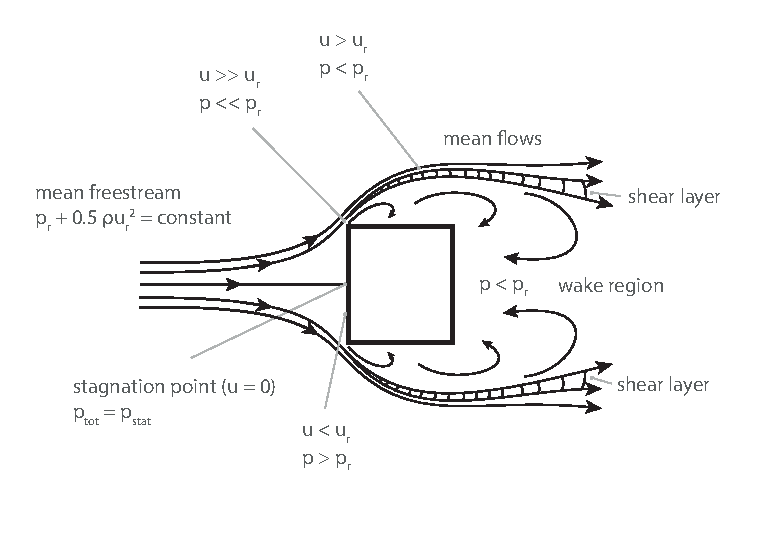
\includegraphics[width=0.9\linewidth, trim= 0cm 1cm 0cm 0cm, clip]{images/flow_around_building}
	\captionsetup{format=plain}%,labelsep=newline}
	\caption[Flow characteristics around a bluff body]{Horizontal section of flow characteristics around a bluff body. The Bernoulli's equation for airflow is valid for the mean flow along a streamline. Adapted from \cite{Aynsley1999}.}
	\label{fig:flowaroundbuilding}
\end{figure}





\subsection{Bernoulli equation}

The Bernoulli equation relates fluid pressure energy, kinetic energy, as well as potential energy of fluid flow along a streamline to each other. It may be considered as a measure of conservation of energy appropriate for fluid flows. Despite small pressure variations, density is considered to be constant for most flows of liquids and gases at low Mach numbers ($Ma \leq \num{0.3}$) \citep{fischer2008experimentelle, Hucho2011}. A further assumption is that the fluid is non-viscous and its flow is steady. The equation for any arbitrary point along a streamline is:

\begin{equation}
p_{tot} = p_{stat} + p_{dyn} + \rho \cdot g \cdot z = constant
\end{equation}

The total pressure refers to the sum of the aforementioned parts. If the variation in temperature is to be neglected or sufficiently small to be ignored, there is no significant change in potential energy along the streamline. Thus,  the above equation reduces to the following simplified form:

\begin{equation}
p_{tot} = p_{stat} + p_{dyn} = constant
\end{equation}

Static pressure is the pressure at a specific point in a fluid acting in all directions. Static pressure can always
be defined, whether or not the fluid is in motion.
Dynamic pressure represents kinetic energy per unit volume of a fluid particle acting in direction of the flow. It is defined as:

\begin{equation}
q = \frac{1}{2} \cdot \rho \cdot u^2
\end{equation}


This equation forms the basis of most air flow calculations used. When using the equation for a streamline around a bluff body, it is evident that the maximum pressure occurs at a point where the flow is brought to rest. This is commonly referred to as the stagnation point. Here, the kinetic energy of the approaching flow is converted into static pressure. Thus, the maximum dynamic pressure is equal to $0.5 \rho u^2$ (see \fref{fig:flowaroundbuilding}).



%The velocity then can be calculated as: 
%
%
%\begin{equation}
%u = \sqrt{ \frac{2 \cdot q}{\rho} }
%\end{equation}



A flow occurs if an opening is placed onto a wall separating two regions of air with different pressure levels.
By evaluating the discharge coefficient, the volumetric flow rate is given by:

\begin{equation}
Q  = S \cdot C_d \cdot A  \sqrt{ \dfrac{2\cdot|\Delta p|}{\rho}}
\end{equation}


where

\begin{equation}
S  = Sign [\Delta p]
\end{equation}

For a rectangular opening, the discharge coefficient $C_d$ is usually assumed to be in the range of \num{0.6} and \num{0.7} \citep{Chu2009}.

%\begin{equation}
%C_d  = \frac{\dot{m}}{A} \sqrt{\frac{\rho}{2\Delta p}}
%\end{equation}

%Rearranging the definition of $C_d$, the flow rate through the opening is given by 

For a cross-ventilation layout with two openings on opposite walls, a more advanced equation can be defined as: 

\begin{equation}
q = \frac{Q}{u_{H} A_{1}} = C_{d_1} \left[ \frac{r_{a}^2 C_{d_r}^2 }{1+ r_{a}^2 C_{d_r}^2} |c_{p_1}-c_{p_2}| \right ] ^\frac{1}{2}
\label{eq:theory:flowrate_advanced}
\end{equation}

where $A_1$ is the opening area of the windward opening, $u_H$ is the external wind velocity at the building height and $c_p$ is the pressure coefficient on the external wall. The ratio of opening areas $r_a$ is defined as  $A_2/A_1$ and the ratio of discharge coefficients is $C_{d_r}  = C_{d_2}/C_{d_1}$, representing the (1) windward and (2) leeward facades, respectively \citep{Chu2014}.
\Fref{eq:theory:flowrate_advanced} can be used to calculate the flow-rate of cross ventilation, though it does not take into account flow resistance caused by furniture or wall friction, which imposes limitations on its usage.

\subsection{Pressure coefficients}
\label{sec:theory:pressure_coefficients}

In order to compare different geometries, it is useful to introduce a normalized pressure coefficient.
The pressure coefficient is a dimensionless number which describes the relative pressures throughout a flow field.  The pressure coefficient at a point near a body is independent of the body size. It is defined as:


\begin{equation}
c_p = {p_{node} - p_\infty \over \frac{1}{2} \rho_\infty u_{\infty}^2 }
\end{equation}



%\begin{equationitem}
%	\item $p_{node}$ is the pressure at the point at which pressure coefficient is being evaluated
%	\item $p_{\infty}$ is the pressure in the free-stream (i.e. remote from any disturbance). In this case it is the static pressure
%	\item $\rho_{\infty}$ is the free-stream fluid density
%	\item $u_{\infty}$ is the free-stream velocity of the fluid
%\end{equationitem}

where
$p_{node}$ is the pressure at the point at which the pressure coefficient is being evaluated,
$p_{\infty}$ is the pressure in the free-stream (free from any disturbance), 
$\rho_{\infty}$ is the free-stream fluid density, and
$u_{\infty}$ is the free-stream velocity of the fluid.
We can also write:

\begin{equation}
c_p = {p_{node} - p_{tot} + q  \over q }
\end{equation}

With this conversion we can say that a $c_{p}$ of \num{0} indicates that the pressure is the same as the free-stream pressure, a
$c_{p}$ of \num{1} indicates the pressure is the stagnation pressure and the point is a stagnation point, and a
$c_{p}$ within $-{\infty} \leq c_{p} \leq 0$  is a significant under pressure region in the flow-field.

%\begin{equationitem}
%	\item $c_{p}$ of 0 indicates the pressure is the same as the free stream pressure.
%	\item $c_{p}$ of 1 indicates the pressure is stagnation pressure and the point is a stagnation point.
%	\item $c_{p}$ within $-{\infty} \leq c_{p} \leq 0$  is significant under-pressure domain in the flow-field
%\end{equationitem}


\subsection{Reynolds number}
\label{sec:reynolds_number}


Turbulent flows face flow separation. 
In order to predict in which condition a flow separation happens, the relative intensity of inertia forces related to the momentum of the moving fluid in terms of its viscous forces needs to be evaluated. This ratio is called the Reynolds number.

%Generally speaking, for Reynolds numbers below 2000, the flow is laminar. For greater numbers $Re_{crit}$ a transition zone occurs until flow happens to be fully turbulent if $Re \gg Re_{crit}$.

When comparing flows around similar geometries with different scales, the Reynolds numbers should be similar. This is important for wind tunnel models, as the geometry is often a limiting factor (cf. \fref{sec:theory:limitations}). 

\subsection{Boundary Layers}
\label{sec:theory:boundary-layer}

The fluid molecules at the surface of solid objects stick to that surface, which leads to shear stress that is caused by the interaction of stationary and moving molecules. The layer between those stationary particles and the point where molecules have reached \SI{99}{\percent} of the free-stream velocity is called boundary layer.

Boundary layers are characterized by their flow properties. For boundary layers where viscous forces are dominant, a laminar flow will be established. For air flows, the laminar boundary layer is very unstable due to the air's low viscosity \cite{Aynsley1999}. The transition from a laminar to a turbulent boundary layer is depicted in \fref{fig:boundarylayer}. The low-law, buffer and viscous sub-regions and their importance is further discussed in  \fref{sec:CFD:boundary_layer}.


\begin{figure}[bht]
	\centering
	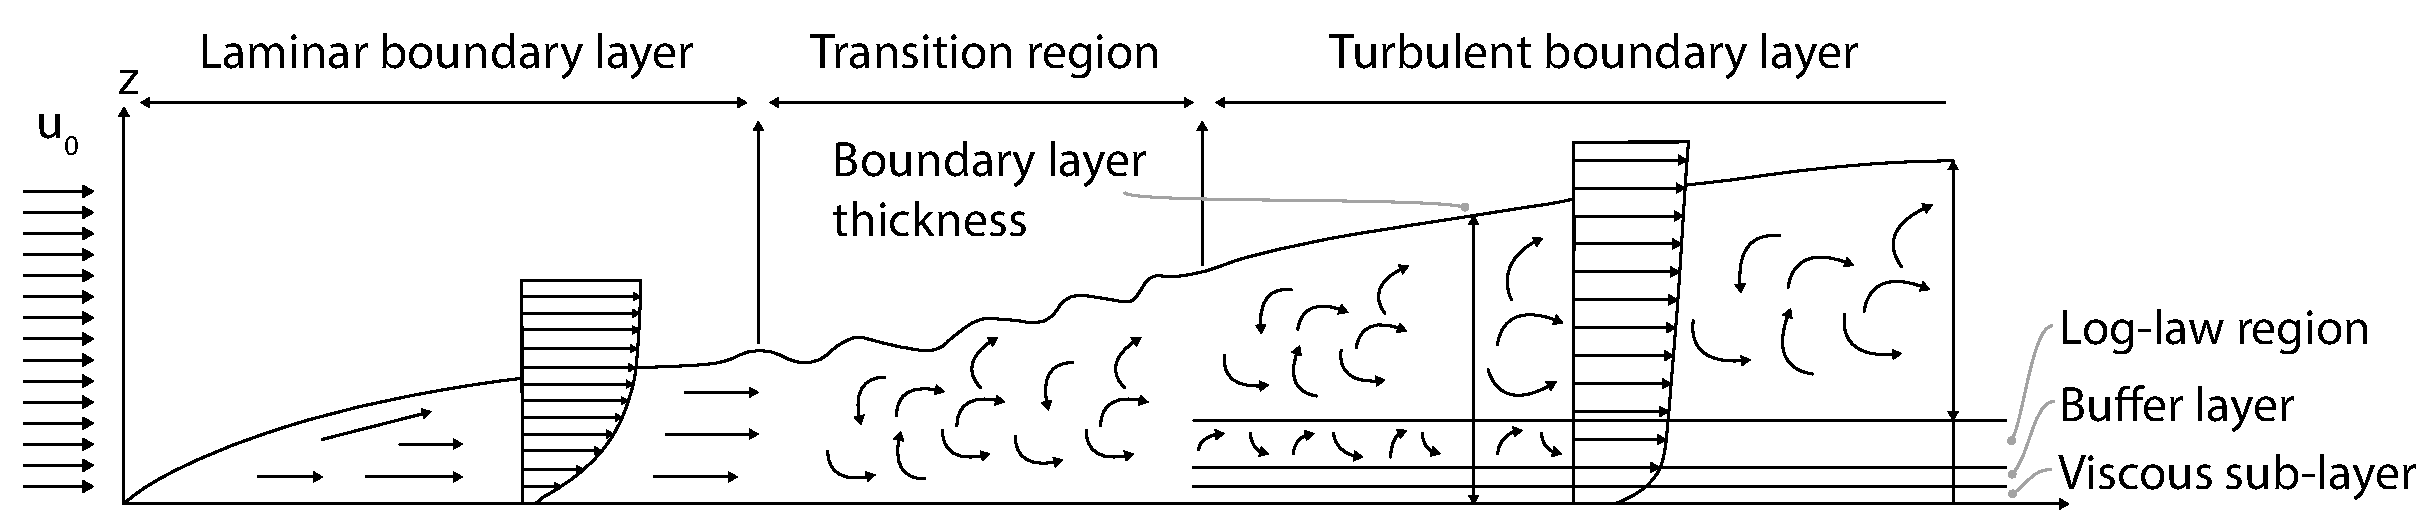
\includegraphics[width=1\linewidth]{images/boundary_layer.pdf}
	\captionsetup{format=plain}
	\caption[Development of a boundary layer over a flat plate]{Development of a boundary layer over a flat plate, including the transition from the laminar to the turbulent region. Adapted from \citep{Cengal2006}.}
	\label{fig:boundarylayer}
\end{figure}









\subsection{Atmospheric boundary layer}
\label{sec:atmABLbasics}

%Wind evolves because of pressure differences. 
%Let $\Delta p$ be a pressure difference of $\Delta p = p_1 < p_2$. As a result, a fluid motion initiated which we call wind. 
On an atmospheric scale, the pressure differences are the result of density gradients which are created by incoming solar irradiation that heats up the surface of the globe in different magnitudes.
The warm air rises which leads to jet streams at an altitude where the ground friction can be neglected.
The further these jet streams reach the earth's surface, the more influence the ground friction has. 
Close to the surface, the roughness of the earth creates a turbulent layer which is called the \gls{ABL}.
\Fref{fig:theory:ABL_example} (a) shows the \gls{ABL} over three types of surface roughnesses, city, suburbia and sea. For each category, the plots ends when $u = \SI{4}{\metre\per\second}$ is reached.



\begin{figure}[!bt]
	\subfloat[][]%
	{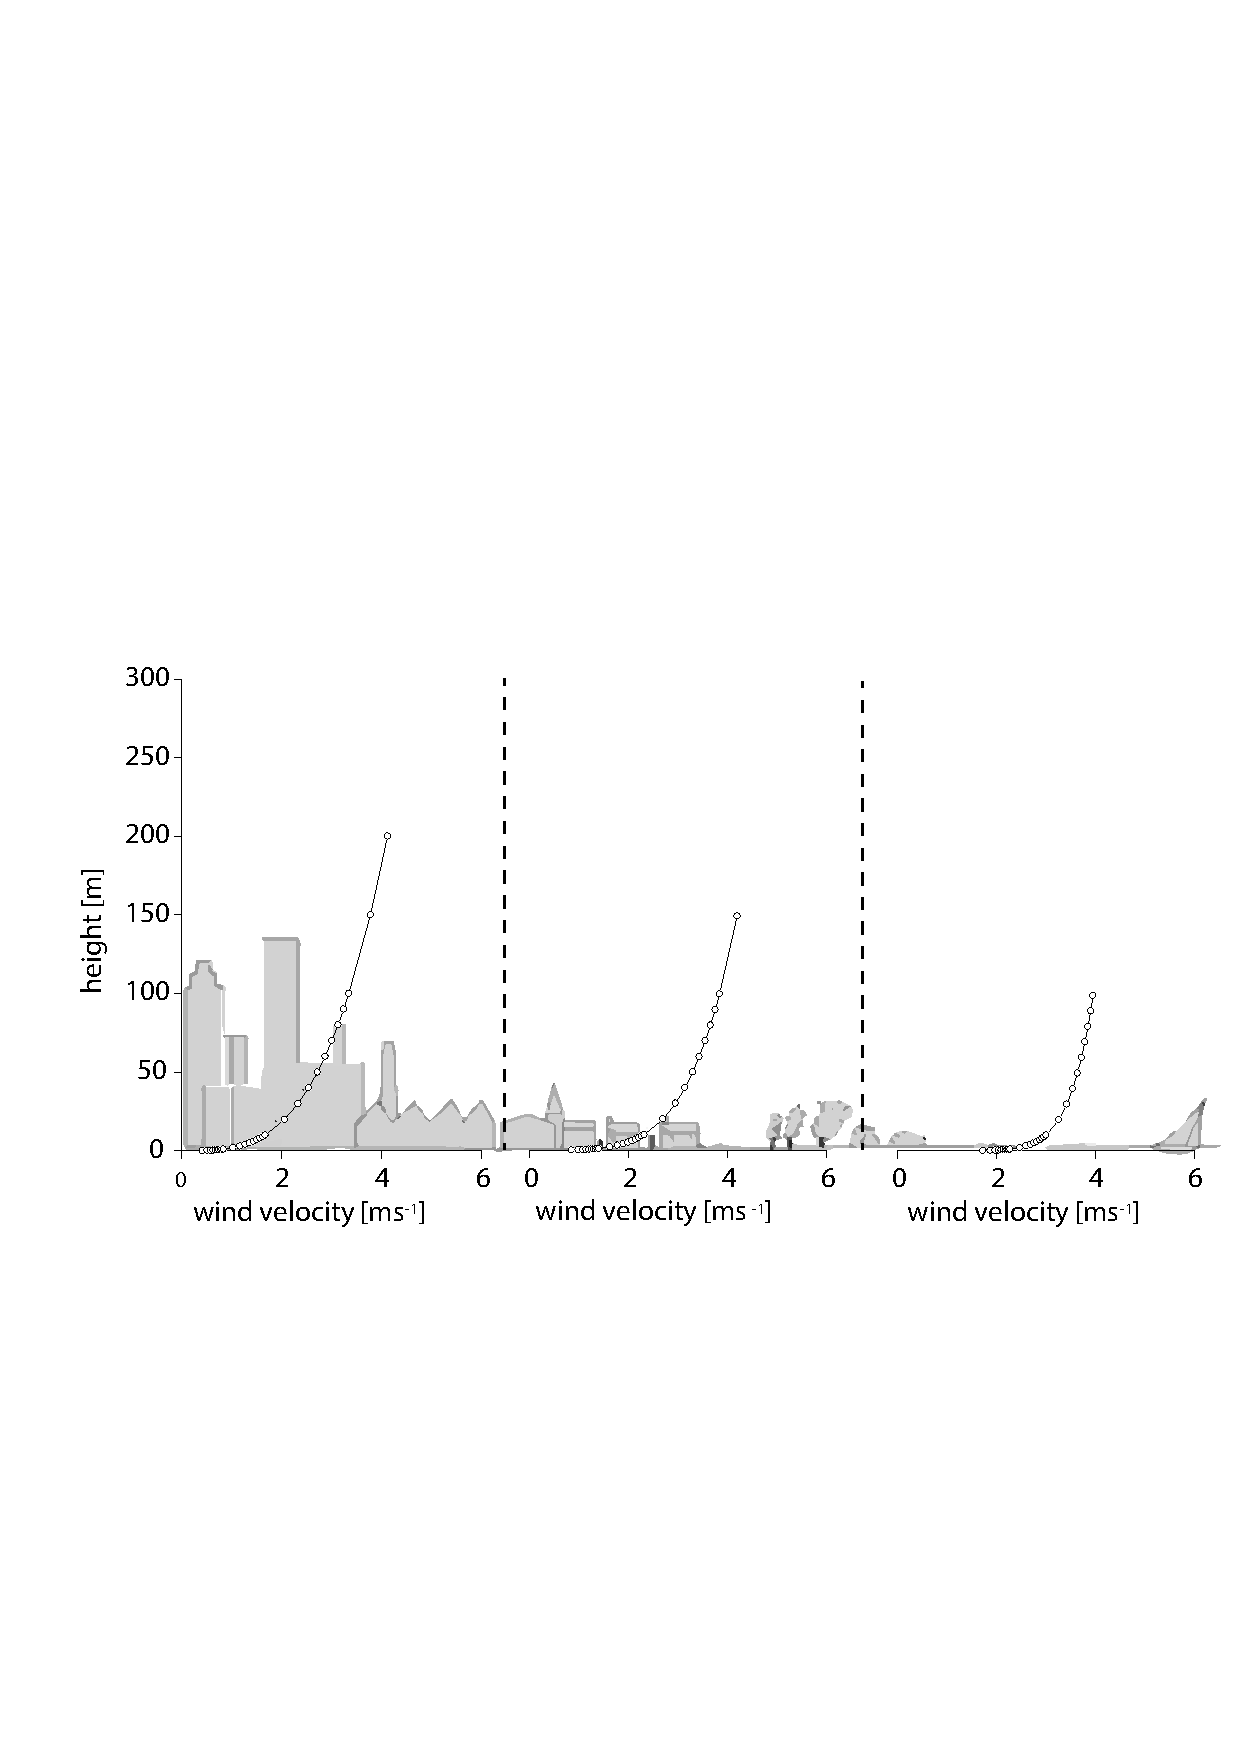
\includegraphics[height=0.4\textwidth, trim = 30 250 35 300, clip=true]{images/atmospheric_boundary_layer_comparison}}
	\subfloat[][]%
	{\includegraphics[height=0.4\textwidth]{images/atmospheric_boundary_layer}}
	\captionsetup{format=plain}
	\caption[Atmospheric boundary layer over three types of surface roughnesses]{Atmospheric boundary layer over three types of surface roughnesses. \textbf{(a)} The \ABL\ over city, suburbia and sea. For each surface, the plots ends when $u = \SI{4}{\metre\per\second}$ is reached. \textbf{(b)} All plots shown up to a height of $\SI{300}{\metre}$ for comparison. }
	\label{fig:theory:ABL_example}
\end{figure}

The wind shear is quantified by the exponent $\alpha$ in the power law equation \ref{eq:power_law} that relates wind velocities at two different altitudes.

\begin{equation}
u(z)=u_{ref}\left( \frac{z}{z_{ref}}\right )^\alpha
\label{eq:power_law}
\end{equation}

%\begin{itemize}
%	\item $\alpha$ is the wind shear exponent 
%	\item $z$ is the height above ground
%\end{itemize}

%where $\alpha$ is the wind shear exponent and
where $z$ is the height above the reference height. The larger the exponent $\alpha$, the larger the vertical gradient in the wind speed. This equation is accurate for altitudes from \SI{100}{\metre} up tp the top of the atmospheric boundary layer. 
For altitudes closer to the ground level, the following logarithmic relation is more applicable \citep{Ghiaus2012,Hucho2011}.

\begin{equation}
u(z) = \frac{u^*}{\kappa} ln \left( \frac{z+z_0}{z_0}\right)
\end{equation}

where \gls{symb:u*} is the \glsdesc{symb:u*}, \gls{symb:kappa} is the \glsdesc{symb:kappa} and \gls{symb:z_0} is the \glsdesc{symb:z_0}. The \glsdesc{symb:z_0}s for different terrains may be found in  \fref{tab:davenport_roughness_class} in the appendix.

Measured wind data have to be converted to a specific site, as wind data is usually collected at airport sites, which correspond to a roughness range of \SIrange{0.0024}{0.03}{} \cite{Ragheb2016}. Translation the data to a specific location is not an easy task because of the irregularities of the urban texture \citep{Ratti2002}.

%\enlargethispage*{3cm}
The \gls{DIN} \citep{DIN10554-2005} suggests a modified profile in which the equation is tailored to certain terrains with the help of the constant $C_{terrain}$. \Fref{tab:boundary_layer_roughness_alpha} shows certain terrain types that can be used with their own specific characteristics described.
Note that the $z_0$ values by \gls{DIN} are not consistent with the ones provided in the appendix, which stresses the point that these are empirical values. 

\begin{equation}
u(z)=C_{terrain} \cdot u_{ref}\left( \frac{z}{z_{ref}}\right )^\alpha
\end{equation}



\begin{table}[hbt]
	\small
	\centering
	\captionsetup{format=plain}
	\caption[Coefficient of terrain for different surface roughnesses]{Coefficient of terrain for different surface roughnesses. Both values are needed to transfer data in a homogeneous site \citep{DIN10554-2005}.}
	\label{tab:boundary_layer_roughness_alpha}
	\begin{tabular}{llSSS}
		\toprule
		Category&  	Description									& {$C_{terrain}$}   & {$\alpha$} 		& {$z_0$} \\
		\midrule
		I 	&	Sea, flat landscape             			& 1.18 				& 0.12     			& 0.01  \\ 
		II 	&	Agricultural landscape         				& 1.0  				& 0.16     			& 0.05  \\ 
		III &	Suburbia, forest              				& 0.77 				& 0.22     			& 0.3   \\ 
		IV 	&	Cities 										& 0.56 				& 0.30    			& 1.0   \\
		\bottomrule
	\end{tabular}
\end{table}

